\scanpage{10}
et par suite on trouve en tous cas
\diagram{\begin{tikzcd}[ampersand replacement=\&,column sep=small,row sep=large]
H^*(X,M)\simeq\&\mathbb H^*(X,\ell Q^*[M])\\
\&E_2^{pq}=H^p(i\mapsto H^q(X,\ell Q^i[M])\arrow[u,Rightarrow]
\end{tikzcd}}

[Sous des conditions convenables, on aura
\[
H^q(X,\ell Q^i[M])=\varprojlim_n H^q(X,Q^i_{\deleted{\unsure{n}}}[M]_{(n)})
\deleted{\unsure{\simeq H^q(X^{\widehat{[i]}},M)}}
\inserted{\simeq H^q(X_{\unsure{n|x}}^{\widehat{[i+1]}},M)}
\]
\margin{\figure{\begin{tikzpicture}[x=1cm,y=1cm]
\node at (0,2.3) {\unsure{Attention}};
\node at (-.7,1.8) {$-$};
\node[draw,ellipse,inner sep=2pt] at (0,1.8) {$+1$};
\node at (0,1.25) {\unsure{nom de|au lieu de} $\widehat{\ }$ !};
\draw (-1.2,.75) .. controls (1.8,.3) and (1.6,2.9) .. (0,2.8) .. controls (-.6,2.8) and (-1,2.65) .. (-1.25,2.55);
\node at (0,.4) {$X^{[i+1]}=[X/S]^{i+2}$};
\node at (0,-.1) {($i+2$ facteurs !)};
\end{tikzpicture}}}
si on écrit
\[
\begin{aligned}
Q^i[M]&=\varprojlim_n Q^i[M]_{(n)}\\
Q^i[M]_{(n)}&=Q^i_{(n)}\otimes_{\underline O_X}M\\
Q^i_{(n)}&=\mathcal P^{\unsure{i+1}}_{(n)}=\cdots
\end{aligned}
\]
].

Si on remplace $M^{\unsure{2|*}}$ par un \uline{complexe} $M^\bullet$ de \deleted{\unsure{$C$}} $D^+(\operatorname{Mod}(X/S))=D^+(X/S)$, on obtient un bicomplexe $Q^*[M^\bullet]$, tel que $\ell Q^*[M^\bullet]$ est une résolution de $M^\bullet$, et par suite
\[
H^*(X,M)\simeq H^*(X,Q^*[M^\bullet])\simeq H^*(X_{\unsure{\mathrm{str}}},\unsure{Q^0(M^\bullet)})
\]
[$Q^0[M^\bullet]$ s'appelle la \uline{\unsure{formalisation}} du complexe \deleted{\illegible{1}} d'op. différentielles $M$.
\margin{\figure{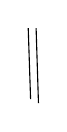
\begin{tikzpicture}[x=1cm,y=1cm]
\draw (0,0)--(-.03,.9);
\draw (.10,-.05)--(.07,.9);
\end{tikzpicture}}}
\margin{9}
